%\chapter{Introducci\'on} % (fold)
%\label{cha:introduccion}
%\addcontentsline{toc}{chapter}{Introducción}



En el nuevo ambiente de las tecnologías de la información cualquier movimiento de almacenamiento masivo puede ser realizado mediante modelos basados en el cómputo nube. \\
El cómputo nube es un término utilizado para nombrar así a la provisión de servicios de almacenamiento a través de Internet que ha sido utilizado para facilitar el cambio de los modelos de negocios, agilizar procesos y reducir costos de operación ~\cite{Nubei}. \\  

Uno de los mayores beneficios que ofrece este servicio es la virtualización de los centros de datos, que pueden operar de manera automatizada, sin necesidad de la presencia de una persona física y pueden ser gestionados en cualquier momento. De acuerdo con un estudio realizado por la consultora Market Research Media, estima que el cómputo nube generará \$270,000 millones de dólares en 2020, por lo que empresas como Google, Amazon, IBM, Oracle y Apple han adoptado este sistema como parte del servicio brindado a sus consumidores, por ejemplo, Google Drive o iCloud, a través de los cuales, con sólo estar conectados a Internet, los usuarios tienen la posibilidad de utilizarlos ~\cite{Nubecomp}. \\ 

Sin embargo, este servicio también presenta algunas desventajas que tal vez nosotros como usuarios no podemos percibir tan fácilmente. Una de ellas es que al almacenar un archivo en realidad no sabemos quién o qué entidades tienen acceso a él. Éste tema se está volviendo cada vez más preocupante sobre todo para instituciones o empresas que cuentan con información confidencial y también debido a diversos ataques por adversarios. \\

Es por eso que se ha optado por la opción del uso de la criptografía, la cual es una ciencia que se encarga del estudio de técnicas para transformar la información a una forma que no pueda entenderse a simple vista; sin embargo, su objetivo no es sólo mantener los datos secretos, sino también protegerlos contra posibles modificaciones o manipulaciones y comprobar la fuente de los mismos  ~\cite{fundamentos}. \\

Ahora bien, la información que circula en dispositivos electrónicos es mayor a la memoria disponible que ofrecen estos, a medida que el volumen de información aumenta, también lo hace la demanda para los servicios de almacenamiento en la nube. Entonces los usuarios tienden a creer que el espacio en la nube es ilimitado y comienzan a guardar grandes cantidades de archivos, por lo cual nos enfrentamos al problema de la duplicación de archivos. \\ 

Es por ello que en el presente documento se propone una solución a estos problemas. Se trata de un protocolo criptográfico que nos brinda la confidencialidad de los archivos a la vez que nos ayuda a evitar la duplicación de los mismos. \\





%\section{Contexto}

%La criptografía es una ciencia que estudia técnicas matemáticas relacionadas con aspectos de seguridad de la información como confidencialidad, integridad de la información, entidades de autenticación y la autenticación de origen de datos entre otras. Esta ciencia tiene como principal objetivo el establecer la comunicación ya sea entre dos personas o dos entidades que requieren compartir información por un canal inseguro el cuál está propenso a un ataque para la manipulación o robo de esta información que viaja en el canal. Es por ello que la criptografía provee de protocolos, algoritmos y demás herramientas que ofrecen una solución para disminuir los ataques no deseados a la información que se requiera compartir de forma segura ~\cite{menezes}.
%\\ \\
%Estos protocolos, algoritmos y técnicas de la criptografía pueden ser utilizadas en distintas áreas de investigación o desarrollo, entre ellas esta el \textbf{Cómputo Nube}. La aplicación de la criptografía en los modelos computacionales basados en el cómputo nube tiene como objetivo proporcionar los algoritmos y protocolos criptográficos que den solución a los problemas en el crecimiento de los grandes volúmenes de información que hoy en día se tienen registro en el servicio de almacenamiento en línea \textbf{(Nube)}, basándose en la eliminación de la información que se encuentre con una copia exacta en la nube. Por ejemplo: 
%\\ \\
%El usuario registrado e identificado dentro de la nube como \textit{Usuario A}, el día de hoy desea almacenar un archivo \textbf{Archivo F} que corresponde a la especificación de los requisitos para la obtención de una beca escolar. Este usuario para no extraviar o modificar el archivo lo almacena en la nube y ahí queda disponible para cuando el lo solicite. Ahora este usuario comparte este archivo mediante un dispositivo \textit{USB} a su amigo ya que este también desea conocer los requisitos para solicitar una beca escolar, este amigo el cuál es otro usuario registrado e identificado dentro de la nube como \textit{Usuario B} también quiere almacenar este archivo \textbf{Archivo F} en la nube, ya que requiere utilizar el espacio de memoria en su dispositivo \textit{USB} para otras actividades y no desea perder los requisitos para la solicitud de su beca escolar. \\
%Ahora en la nube se encuentran almacenados 2 copias del \textbf{Archivo F} por dos diferenes usuarios identificados como  \textit{Usuario A} y \textit{Usuario B}, ambos almacenaron el mismo archivo en el mismo lugar, sin darse cuenta que ahora este archivo se encuentra duplicado en la nube. 



%Según un estudio realizado por Mundo de la informática (una revista mundial reconocida por su enfoque a las tecnologías de la información y comunicación) a empresas de tecnologías de la información, aseguran que el 42\% de estas empresas de TI están planeando aumentar el gasto en cómputo nube, siendo el crecimiento mayor en las empresas con más de 1000 empleados (52\%). Las 5 áreas de mayor crecimiento se ilustran en la figura ~\ref{fig:1-1-1}

%\begin{figure}[H]
%\centering
%	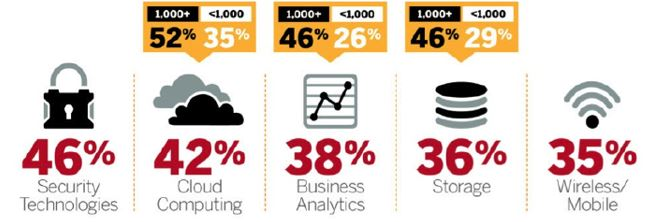
\includegraphics[width=15cm, height=5cm]{./images/aumentoCloudComputing.jpg}
%	\caption{Aumento del gasto por las empresas en cómputo nube}
%	\label{fig:1-1-1}
%\end{figure}


%El cómputo nube es un término general utilizado para nombrar así a la provisión de servicios de almacenamiento a través de internet que ha sido utilizado para facilitar el cambio de los modelos de negocios, agilizar procesos y reducir los costos de operación en las grandes empresas u organizaciones. 

%De acuerdo con un estudio realizado por la consultora Medios de investigación de mercado \textit{(Market Research Media)}, el cómputo nube generará \$270,000 millones de dólares en 2020, por lo que empresas como Google, Amazon, IBM, Oracle y Apple han adoptado este sistema como parte del servicio brindado a sus consumidores, por ejemplo Google Drive o iCloud, a través de los cuales, con sólo estar conectados a Internet, los usuarios tienen la posibilidad de utilizarlos ~\cite{Nubecomp}. \\ \\ 

%Básicamente el almacenamiento en la nube se caracteriza por 5 puntos esenciales que son: 
%	\begin{itemize}
%		\item \textbf{Autoservicio on-demand o pago por evento}  
%		\item \textbf{Acceso ubicuo a la red (uso de los servicios cuando sea y donde sea)}  
%		\item \textbf{Fondo común de recursos} 
%		\item \textbf{Rápida elasticidad} 
 %		\item \textbf{Servicio medido}  ~\cite{Compnube}.
 %\end{itemize}



\section{Planteamiento del problema.}
Hoy en día millones de personas en el mundo tienen la facilidad de acceder a un dispositivo electrónico que les permite manipular información o almacenarla ya sea en un dispositivo físico o en la nube.
Debido a los limitados recursos financieros y altos gastos de almacenamiento de datos electrónicos, los usuarios prefieren almacenar sus datos en los entornos de nube provocando enormes demandas a las compañías que ofrecen este servicio. El incremento en el uso de estos servicios implica que los sistemas de almacenamiento tengan más capacidad y puedan cubrir la alta demanda que se presenta en el mercado ~\cite{Keelveedhi}. \\

%Ahora bien, la información que circula en dispositivos electrónicos es mayor a la memoria disponible que ofrecen estos, a medida que el volumen de información aumenta, también lo hace la demanda para los servicios de almacenamiento en línea ~\cite{Bellare}. Un gran incremento en el uso de estos servicios implica tener más infraestructura y personal para que los sistemas de almacenamiento tengan más capacidad y puedan cubrir la demanda que se presenta en el mercado. Si bien el almacenamiento logró dar buenos resultados al cliente en sus primeras etapas, ahora la preocupación por el incremento de infraestructura para seguir dando esos resultados se ha incrementado considerablemente  ~\cite{Keelveedhi}.
%\\ 

Para entender un poco más acerca de la problemática a la que se enfrenta el almacenamiento en la nube, mostramos el siguiente estudio realizado por EFE/Cisco: \\ 

EFE/Cisco realizó una estimación en el año 2014 en su cuarto informe anual Índice Global sobre la nube (2013-2018), donde prevé que en 2018 la mitad de la población mundial tendrá internet en sus hogares y más de la mitad almacenará contenidos en servicios personales de almacenamiento en la nube. El estudio adelanta que se triplicará el crecimiento de tráfico en los centros de datos en los próximos cinco años y la nube representará el 76\% de ese total, mientras que en 2013 éste solo representaba el 54\%, lo que supondría un aumento anual de 32\%. El tráfico en centros de datos, contando el saliente a usuarios finales, entre centros y dentro del propio sistema superará los 3.1 zettabytes de 2013 y llegará a los 8.6 que se esperan registrar en 2018, suponiendo una tasa anual del 23\% ~\cite{cisco}. 
\\ 
En 2018, el 53\% de los usuarios de internet con red doméstica usarán servicios de almacenamiento en la nube, aportando un tráfico medio por usuario de 811 Mb mensuales, lejos de los 186 Mb de 2013. Además, se espera, según la nota que publicó Cisco, que en 2018 el 69\% de la carga de trabajo en la nube se realizará en centros de datos con nubes privadas, un dato que fue del 78\% en 2013. El resto de cargas de trabajo, el 31\%, se realizarán en la nube pública, subiendo desde el 22\% del 2012 ~\cite{cisco}. Crecimiento en el tráfico de información en la nube ~\ref{fig:1-2-1} \\

\begin{figure}[H]
\centering
	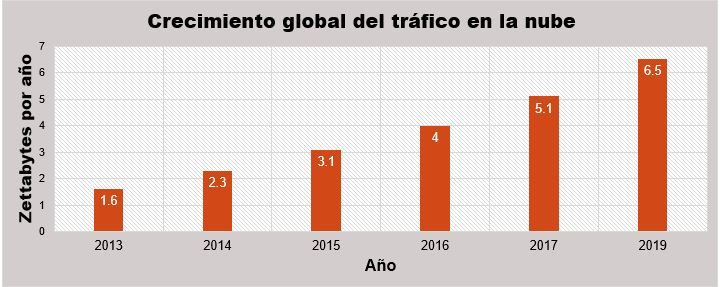
\includegraphics[width=13cm, height=5cm]{./images/crecimientoNube.jpg}
	\caption{Crecimiento global del tráfico en la nube}
	\label{fig:1-2-1}
\end{figure}

Una de las principales razones del incremento en el tamaño en la estructura de almacenamiento de servicios en línea es la duplicación de archivos, existen muchas copias en la nube de un mismo archivo que se encuentra presente en diferentes cuentas de usuarios. Un ejemplo: El usuario registrado e identificado dentro de la nube como \textit{Usuario A}, el día de hoy desea almacenar un archivo \textbf{Archivo F} que corresponde a la especificación de los requisitos para la obtención de una beca escolar. Este usuario para no extraviar o modificar el archivo lo almacena en la nube y ahí queda disponible para cuando él lo solicite. Ahora este usuario comparte este archivo mediante un dispositivo \textit{USB} a su amigo ya que este también desea conocer los requisitos para solicitar una beca escolar, este amigo el cuál es otro usuario registrado e identificado dentro de la nube como \textit{Usuario B} también quiere almacenar este archivo \textbf{Archivo F} en la nube, ya que requiere utilizar el espacio de memoria en su dispositivo \textit{USB} para otras actividades y no desea perder los requisitos para la solicitud de su beca escolar. \\

Ahora en la nube se encuentran almacenados 2 copias del \textbf{Archivo F} por dos diferentes usuarios identificados como \textit{Usuario A} y \textit{Usuario B}, ambos almacenaron el mismo archivo en el mismo lugar, sin darse cuenta que ahora este archivo se encuentra duplicado en la nube. \\

Otro punto importante es la seguridad e integridad de la gran cantidad de información que se almacena en la nube. Este servicio de almacenamiento está sujeto a los ataques de adversarios que están interesados en el robo, manipulación o alteración de la información. Uno de los ataques que se han intentado realizar por dichos adversarios es el ataque por fuerza bruta, el cual es una forma de recuperar una clave probando todas las combinaciones posibles hasta encontrar aquella que permite el acceso al archivo. 
 \\  \\



%\section{Justificación}

%En la actualidad millones de personas usan los servicios de almacenamiento que ofrece la nube, ya sean gratuitos o privados, este número de personas ha ido en un incremento exponencial lo cual hace que el espacio de almacenamiento disminuya, entonces ¿Cómo podría mitigar el problema de almacenamiento y tener privacidad de los datos al mismo tiempo.\\

%Usando la criptografía clásica para poder cifrar un archivo se utiliza una clave privada la cuál es distinta para cada usuario, cada vez que se cifra un archivo el resultado de este es diferente para cada intento. Por tanto no se puede evitar la duplicación de archivos utilizando este mecanismo de la criptografía y se deben implementar soluciones más robustas.

%Una solución para tener privacidad y evitar duplicación la proporcionó John R. Douceur, la cual dice que teniendo a M que será el contenido de un archivo de aquí en adelante denominado el mensaje, el cliente primero calcula una clave K ← H(M) mediante la aplicación de una función de hash criptográfica H al mensaje y luego calcula el texto cifrado C ← E(K,M) a través de un esquema de cifrado simétrico determinista. El derivado del mensaje K se almacena por separado cifrándolo con una llave por cliente. Un segundo cliente B cifra el mismo archivo M que producirá el mismo C, evitando la duplicación ~\cite{donceur}. \\

%En el artículo publicado por Mihir Bellare, Sriram Keelveedhi, Thomas Ristenpart, nombrado “DupLESS: Server-Aided Encryption for Deduplicated Storage” ~\cite{Bellare}, se observó que uno de los principales problemas al que nos enfrentamos es que el esquema de cifrado solo es seguro cuando el espacio de mensajes es demasiado grande, por lo tanto agentes externos pueden provocar agravios a la integridad de la información de los usuarios.

%Si bien esta solución se ocupa de la duplicación de archivos deja muy vulnerable el aspecto de la privacidad, ya que ante un espacio de mensajes pequeño las amenazas del adversario son demasiadas. Si se tuvieran como ejemplo 1000 mensajes, para el adversario sería muy fácil intentar encontrar la clave, probando las 1000 claves posibles generadas con la función hash, hasta descifrar el archivo, por lo tanto se comprueba que un espacio de 1000 mensajes sigue siendo pequeño.

%Es por ello que este trabajo terminal tiene como principal meta atacar esta problemática de privacidad, proponiendo una arquitectura del sistema que a través de un servidor de llaves se generaran llaves de acuerdo al contenido del archivo, para con esta se pueda cifrar y luego almacenar en la nube donde se eludirá la duplicación de archivos. 



\section{Propuesta de solución. }

Como se mencionó anteriormente encontramos dos principales problemas, uno es la confidencialidad de los archivos cuando se almacenan en la nube y el otro es la cantidad de archivos duplicados en la misma. \\

Para combatir el problema de la confidencialidad, proponemos el uso de la criptografía, a cada usuario se le proporcionará una llave con la que puede cifrar y descifrar archivos, pero no podemos usar criptografía de manera tan simple ya que si dos usuarios cifran el mismo archivo daría como resultado dos archivos cifrados distintos, entonces al hacer la comparación de ambos archivos no habría forma de atacar el problema de la duplicación de archivos. Así que nos encontramos con otro problema, pues evitamos que los archivos estén expuestos a adversarios, pero seguimos con el problema de archivos duplicados.\\

 Por lo tanto, nos basaremos en el protocolo denominado DupLESS el cual combina varias herramientas criptográficas de tal forma que se pueda tener un control de las llaves relacionadas con los archivos y los usuarios sin comprometer el contenido e integridad de la información, de esta manera si dos usuarios quieren cifrar el mismo archivo obtendrán la misma llave. Por consiguiente, al cifrar los archivos obtendríamos como resultado el mismo archivo cifrado, esta vez al hacer la comparación se detectará la duplicación de archivos y únicamente se guardará una copia del archivo, ahorrando espacio de memoria y costos de infraestructura. \\

Como se observa en la siguiente figura ~\ref{fig:1-3-1} varios usuarios realizan peticiones para subir archivos, pero se puede notar que algunos son iguales, por lo que pasan por un proceso de eliminación de duplicados antes descrito y finalmente se almacena una copia de cada uno. \\




%La eliminación de duplicación de datos es una técnica que avanza favorablemente y da como resultado la disminución drástica de la cantidad de información duplicada en la nube, cuando esta se elimina del almacenamiento. En general, la eliminación de duplicados compara la información nueva que se requiere almacenar con la información que ya se tiene archivada y elimina las duplicaciones en la nube reduciendo la asignación de almacenamiento dentro de esta, esta disminución en la nube puede reducir las necesidades de almacenamiento en hasta un \textit{80\%} para archivos y copias de seguridad que los usuarios resguardan en la nube como se ilustra en la figura ~\ref{fig:1-3-1}. Las ventajas de no tener duplicados en la nube incluyen una mayor capacidad de almacenamiento y ahorro presupuestario, al igual que la minimización del ancho de banda para menos costosa y más rápida la repetición de la información fuera de la reserva simplificando y mejorando la gestión del almacenamiento de datos  ~\cite{rededup}. 

\begin{figure}[H]
\centering
	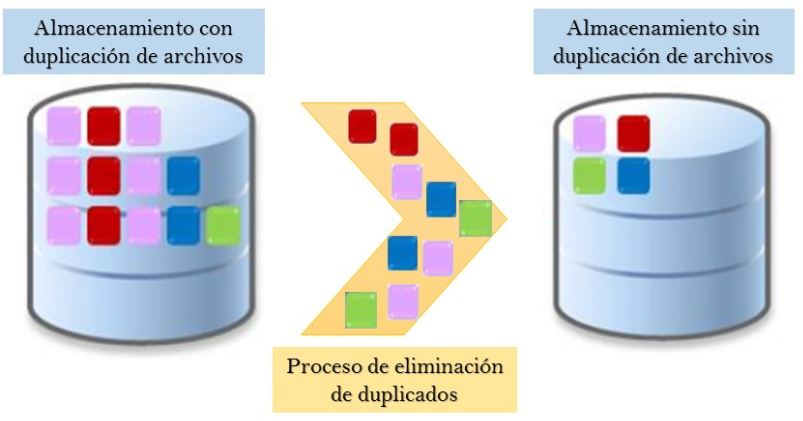
\includegraphics[width=10cm, height=5cm]{./images/Deduplicacion.jpg}
	\caption{Eliminación de Duplicados}
	\label{fig:1-3-1}
\end{figure}

%Una posible solución para la protección a los datos y eliminación de duplicaciones, es echar mano de la criptografía. Ciencia que se encarga del estudio de técnicas para transformar la información a una forma que no pueda entenderse a simple vista; sin embargo, el objetivo de la Criptografía no es sólo mantener los datos secretos, sino también protegerlos contra la modificación o manipulación y comprobar la fuente de los mismos ~\cite{fundamentos}. \\   \\
%Está ciencia que mantiene la información segura se encuentra dividida en dos grandes tipos: \textbf{Criptografía Simétrica} y \textbf{Criptografía Asimétrica}.  \\

%\textit{La criptografía simétrica} o también llamada criptografía de llave secreta, basa su seguridad en una sola llave que se comparte entre dos entidades que quieren compartir información, dicha llave es utilizada para cifrar un archivo al ser enviado a la otra entidad y este utilizará la misma llave para descifrarlo cuando lo reciba. \\
%\textit{La criptografía asimétrica} o criptografía de llave pública involucra el uso de un par de llaves para cada entidad que desea comunicarse, estas llaves llamadas pública y privada. Para que una entidad envíe un archivo a otra, necesita cifrar el archivo con la llave pública de esa entidad a la que se desea enviar, y cuando lo reciba esa entidad lo deberá descifrar con su llave privada o secreta. De esta manera se evita el compartir llaves para cifrar y descifrar como sucede en la criptografía simétrica y reduce los riesgos de un ataque de adversarios.  \\ \\


%El objetivo de esta propuesta de solución es almacenar más datos en menos espacio mediante el uso de la criptografía. Esta ciencia nos proveerá con sus herramientas para la creación de un llavero criptográfico, dicho llavero realizará una firma la cuál dará paso a la creación de una llave correspondiente a un archivo \textit{F} que se desee almacenar un usuario, si se llega a solicitar al llavero por un usuario diferente una nueva firma para la creación de una llave para el mismo archivo \textit{F}, esta llave será la misma, ya que el mecanismo de funcionamiento entre un usuario y este servidor está diseñado para que sea capaz de identificar el mismo archivo sin comprometer el contenido e integridad de este. Esta  llave va a lograr que cuando se cifre este archivo por \textit{n} cantidad de usuarios diferentes que lo poseen, dicho cifrado será igual para la \textit{n} cantidad de usuarios, permitiendo así que en la nube al subir estos cifrados se realice una comparación para que reconozca a quien pertenecen esos cifrados y sólo tenga almacenada una sola copia de este, ahorrando espacio de memoria y costos de infraestructura. 

%Puesto que ambas cuestiones, la eliminación de duplicados y la privacidad de la información, son importantes, se ha comenzado a
%proponer mecanismos que solucionen ambos problemas de manera conjunta, que son: Dupless ~\cite{Bellare}, ABS: the apportioned backup
%system. ~\cite{abs}, Flud Backup ~\cite{flud}, SIGOPS Oper. Syst. ~\cite{sigops}, TahoeFS ~\cite{tahoe}.


\section{Objetivos. } % (fold)

    \subsection{Objetivo General.} % (fold)
    Desarrollar un protocolo criptográfico para evitar la duplicación de archivos almacenados en la nube, garantizando la privacidad de los usuarios contra adversarios cuando el espacio de mensajes es pequeño, utilizando algoritmos criptográficos para su implementación. 
     
    \subsection{Objetivos Específicos.} % (fold)
	\begin{itemize}
		\item Evitar la duplicación de archivos que sean almacenados por los usuarios de la nube
		\item Proteger ante los adversarios la información de los usuarios de la nube
		\item Establecer un esquema de autenticación de usuarios 
		\item Reducir la pérdida y filtración de información de los usuarios de la nube
		\item Evitar los ataques por fuerza bruta al contenido de los archivos de usuarios en la nube. 
 	\end{itemize}

\section{Organización del documento. }

El presente documento que detalla todo el proceso de creación de este protocolo criptográfico está conformado por 6 diferentes capítulos los cuáles son: 

\begin{itemize}
	\item Capítulo 1 \textbf{Introducción} \\
                     En este capítulo se expone cuál es el contexto en el que este trabajo terminal se desarrollará, así mismo se describe cuá a sido la problemática detectada a partir del análisis del contexto en el cuál se desarrola la investigación y finalmente se muestran cuales son los objetivos tanto general como específicos de este trabajo terminal, es decir, cuál es la finalidad de éste protocolo criptográfico. 

	\item Capítulo 2 \textbf{Marco Teórico} \\
El contenido de este capítulo abordará temas estrechamente relacionados con la criptografía y la seguridad de la información. También, este capítulo contiene información acerca de los 2 tipos de criptografía que existen mencionando los diferentes esquemas de cifrado y los modos de operación que son utilizados por algunos de estos. De igual forma se describe con detalle los servicios que ofrece el cómputo nube. 

	\item Capítulo 3 \textbf{Estado del Arte} \\
	En dicho capítulo se encontrará plasmada una comparativa realizada entre sistemas o prototipos que tienen una similitud con el protocolo criptográfico que este trabajo terminal propone. Esta comparativa contendrá detalles técnicos enfocados a las herramientas criptográficas utilizadas en estos sistemas.

	\item Capítulo 4 \textbf{Protocolo Dupless} \\
            El capítulo 4 contiene a gran detalle el funcionamiento del protocolo criptográfico Dupless, dicho protocolo será la base de la investigación para el desarrollo de este trabajo terminal. 

	\item Capítulo 5 \textbf{Análisis} \\
	Como otro capítulo más de este documento se encuentra el análisis del protocolo criptográfico, el cuál se compone de la realización de un estudio de factibilidad y análisis de riesgos para la realización de este proyecto, asimismo se muestra cuál será la arquitectura de trabajo terminal, la descripción de todos los procesos que involucrán la creación de este protocolo, el modelo de entidades que comprende diagrama entidad relación y el diagrama de clases para su implementación. Al final de este capítulo se podran encontrar los requerimientos de este protocolo criptográfico tanto funcionales como no funcionales y las reglas de negocio que lo componen.

	\item Capítulo 6 \textbf{Diseño} \\
	El capítulo de diseño tiene como contenido la especificación de la plataforma del protocolo, es decir, la especificación de recursos necesarios para poder llevar a cabo su implementación con las herramientas necesarias, y también todos los casos de usos que involucran el funcionamiento de dicho protocolo.

\end{itemize}




    